\section{The Super High Momentum Spectrometer (SHMS)}

The Super High Momentum Spectrometer (SHMS) operates on the beam-left
side of the beamline, and can be rotated around the pivot for scattering angles from 5.5
to 40~degrees. It was built between 2009 and 2016 as the major
Hall-C component of the 12-GeV Upgrade Project.  The five superconducting
magnets on the SHMS can be set for a central-ray momentum of up to 11~GeV/c.
The minimum design momentum is 2 GeV/c. A CAD model of the SHMS is shown
in Fig.~\ref{fig:SHMS_CAD_Model}, and Table~\ref{tab:shms_specs} lists the performance specifications.

\begin{figure}
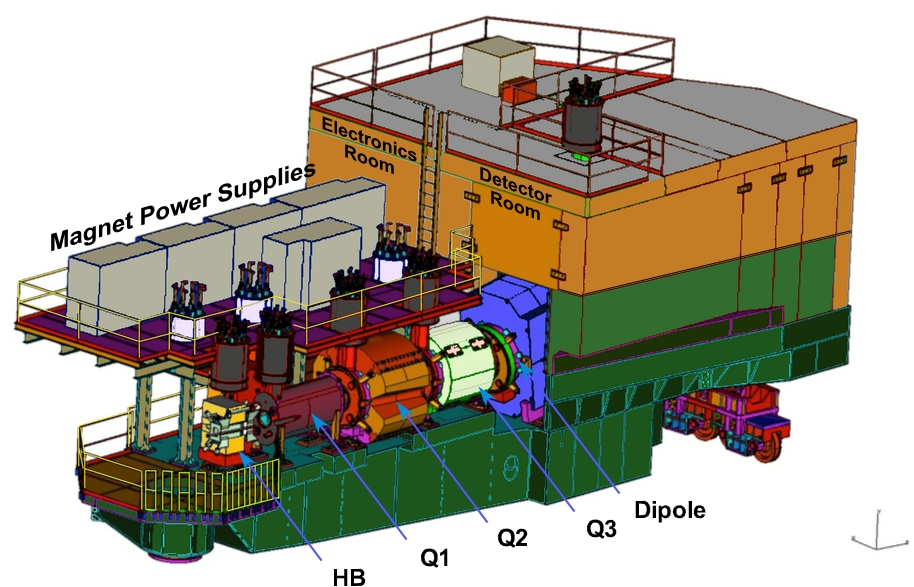
\includegraphics[width=6in]{SHMS_Rendered_Recolored_Annotated}
\caption{CAD Rendering of the Super-High-Momentum Spectrometer. \label{fig:SHMS_CAD_Model}}
\end{figure}

\begin{table}
\begin{center}
\caption{SHMS Design Parameters\label{tab:shms_specs}}
\vspace{\baselineskip}
\begin{tabular}{|l|l|}
\hline
Parameter						& SHMS Design 			\\ \hline
Range of Central Momentum		& 2 to 11 GeV/c for all angles	\\
Momentum Acceptance $\delta$	& $-10\%$ to $+22\%$			\\
Scattering Angle Range			& 5.5 to 40 degrees			\\
Solid Angle Acceptance			& $>$ 4.0 millisterradians		\\
Horizontal Angle Resolution		& 0.5 - 1.2 mrad			\\
Vertical Angle Resolution			& 0.3 - 1.1 mrad			\\
Vertex Length Resolution			& 0.1 - 0.3 cm				\\
Tracking Rate Capability			& 5 MHz					\\
Beam Capability				& Up to $90 \mu$A			\\
\hline
\end{tabular}
\end{center}
\end{table}


The primary magnetic elements on the SHMS, the Q1, Q2, Q3, and Dipole magnets, provide
point-to-point focusing and momentum dispersion just like the four magnets with
the same names on the HMS. The dipole of the SHMS bends central-momentum particles
trajectories up by $18.2^{\circ}$. The SHMS Q1 was
manufactured by Scientific Magnetics, Inc. in Abingdon, England. Q2, Q3, and
the Dipole were constructed by Sigmaphi in Vannes, France.

In order to reach the smallest scattering angles, the SHMS has a horizontally-bending dipole
magnet as its first magnetic element. Referred to as ``HB", it was built by FRIB, the Department of Energy
facility at Michigan State  University. This small, high-field magnet bends
central-momentum particles to the left by 3~degrees so that the remainder of the
spectrometer parts will be further away from the primary electron beam. The HB
magnet is an asymmetric ``C''-dipole which has a flux-return iron yoke only on
the side away from the primary beam. When the SHMS is set for small scattering
angles, the electron beam passes very close to the spectrometer and to the
HB magnet's superconducting
coils. In this configuration the coils see a high radiation dose which may cause
them to have a limited
lifetime. Experiments must be planned in such a way that this exposure is minimized.

A further consequence of making the SHMS operate at small scattering angles is
that the iron yokes of the HB and Q2 magnets had to be designed with notches
that just clear the beamline vacuum pipe. The fringe fields from these magnets can
deflect the primary electron beam away from the middle of the beam dump.
The effects of this field
must be mitigated by a combination of good experiment planning, magnetic shielding,
and automatic safety systems.

The SHMS shield house has two rooms. The dipole magnet penetrates the front
wall of the room containing the detectors. Inside this are the two sets of 6-plane
drift chambers, the Heavy-Gas Cherenkov (HGC), the two pairs of trigger hodoscopes
(S1X/S1Y and S2X/Q2Y), and
the Preshower and Shower Counters (calorimeters). The SHMS focal plane forms an
angle of about 5~degrees with respect to the central trajectory,
and intersects that trajectory at
a point midway between the two drift chamber boxes. Additional  particle-identification
detectors (Noble-Gas Cherenkov (NGC), and/or Aerogel Cherenkov) may also be
installed if needed by the current experiment. When the NGC is not in use it may
be replaced by a tank that extends the vacuum system up  to a window just in
front of the first drift chamber. In this configuration, a mechanical safety shutter
must be closed over this large vacuum window before personnel may enter the
room.

The second room in the SHMS shield house houses the
electronics controlling the magnet power supplies, the data-acquisition
electronics (DAQ) and power supplies for the detectors, and theVESDA
smoke and flammable gas sensor systems. When personnel enter the shield
house they first pass into this "Electronics Room".

